%\documentclass[12pt,thmsa]{article}

\documentclass[11pt]{article}
\usepackage[spanish]{babel}  
\usepackage[utf8]{inputenc} 
\usepackage{amsmath}
\usepackage[pctex32]{graphicx}
\usepackage{amsfonts}
\usepackage{enumerate}
\usepackage{color}
\usepackage[normalem]{ulem} %%%% para tachar texto
\usepackage{setspace} %% interlineado
\usepackage{float}
\usepackage{multirow}
\usepackage{booktabs}

\onehalfspacing

\usepackage{siunitx}

\usepackage{fouriernc} %%% Fuente más legible
\usepackage{merriweather} %%% Fuente más legible

\usepackage{geometry}
\geometry{
	a4paper,
	total={170mm,257mm},
	right=20mm,
	left=20mm,
	top=20mm,
	bottom=20mm
}

\title{\textbf{Teoría estadística de la información \\en el procesamiento de imágenes y señales}}
\date{}
\begin{document}
	
	\maketitle

%-----------------Introducción
\section{Resumen}
La utilización de conceptos relacionados con la teoría de la información combinados con técnicas estadísticas, aplicados al procesamiento de imágenes y señales ha ganado mucho espacio en los últimos tiempos. Medidas de discriminación estocástica como son las $(h,\phi)$ divergencias y las $(h,\phi)$ entropías han sido aplicadas al problema de estimación de parámetros, detección automática de bordes y medidas de contraste entre otras aplicaciones. 

\textcolor{red}{Este proyecto se propone estudiar la eficacia que tienen las medidas de divergencia propuestas asociadas tanto a imágenes provenientes de radares de apertura sintética (SAR) en el contexto del diseño de nuevos métodos de filtrado y de clasificación, como al análisis estadístico de características estelares estudiando la distribución de la velocidad de rotación de ciertos grupos de estrellas. }


Las imágenes SAR son muy ruidosas debido a la presencia del ruido speckle que es característico de tecnologías que emplean sistemas de iluminación coherente como el laser, microondas, ultrasonido entre otras. Este ruido causa un patrón granular que dificulta el análisis e interpretación de estas imágenes, y puede conducir a una reducción en la precisión de los algoritmos de clasificación y de segmentación. 

En este contexto se analizarán y llevarán adelante estrategias que incluyan la aplicación de estas medidas en el diseño e implementación de nuevos algoritmos de clasificación y de filtrado de este tipo de imágenes. Como resultado de este estudio se implementarán rutinas computacionales que puedan ser utilizadas en la aplicación a imágenes reales.

Asimismo, este proyecto estudiará la factibilidad de utilizar estas medidas en astroestadística,  dado que la estimación de funciones de distribución de características estelares como la clasificación de espectrogramas es un problema de interés en la actualidad.



%Esta propuesta se abordará  estudiando la eficacia que tienen las medidas de divergencia propuestas asociadas a una imagen SAR en el contexto del diseño de nuevos métodos de filtrado y de clasificación. 



\section{Estado del arte}
%La teledetección constituye una herramienta de gran utilidad para el desarrollo
%de sistemas de prevención, seguimiento y evaluación de superficie terrestre.
%Se define como las técnicas que permiten adquirir imágenes (y otras formas de
%organizar datos: señales, series de tiempo, etc.) de la superficie terrestre desde
%sensores instalados en plataformas espaciales o aerotransportadas.

%%% ACF Acá asociás clasificación a textura, en general. La clasificación, en general, trata de discriminar áreas con atributos diferentes. La textura entra después que presentes SAR, y digas que es sensible a la textura.
El problema de clasificación de una zona de una superficie terrestre en clases es uno de los objetivos fundamentales en teledetección debido a que esto posibilita detectar zonas de inundación, de incendios, de derrame de petróleo tan importantes en el monitoreo ambiental. 
Por este motivo el desarrollo de algoritmos de clasificación y de interpretación automática de imágenes cobra vital importancia  ya que permite determinar áreas en la imagen con características comunes  y producir un mapa temático de la región. 

%Los algoritmos de clasificación pueden dividirse en no supervisados y supervisados. En los primeros no se necesita que el algoritmo interactúe con el usuario ya que éste realiza una búsqueda automática de grupos con características semejantes dentro de la imagen. Los segundos requieren de muestras de entrenamiento definidas por el usuario donde se conoce la clase a la cual pertenecen. Estas muestras serán utilizadas para asignar píxeles con clasificación desconocida. En ambos algoritmos la extracción de características que permitan una clasificación precisa juega un rol de suma importancia.
Las imágenes adquiridas con radares de apertura sintética (SAR) juegan un papel preponderante en el sensado remoto debido a sus ventajas respecto de las adquiridas por sensores ópticos. La independencia de las condiciones climáticas y de la iluminación junto con la capacidad de penetrar la nubes, las copas de los árboles e incluso el suelo, han contribuido para que resulten cada vez más populares. 

En particular, en Argentina la Comisión Nacional de Actividades Espaciales y el INVAP junto con otras agencias internacionales, forman parte de la misión SAOCOM. Esta misión consiste en la puesta en órbita de satélites equipados con tecnología para adquirir imágenes SAR con el objetivo de medir de la humedad del suelo, detectar derrames de hidrocarburos en el mar y el seguimiento de la cobertura de agua en las inundaciones. 


Sin embargo, este tipo de imágenes tiene la desventaja de ser difícil de interpretar y procesar por la presencia del ruido speckle. 
Este ruido es inherente al proceso de captura de la imagen y se hace presente debido a la superposición coherente de las ondas reflejadas por muchos dispersores. Esto causa una variación en la intensidad píxel a píxel que se manifiesta en la imagen como un patrón granular que dificulta su análisis e interpretación. 
Por este motivo la utilización de modelos estadísticos y el desarrollo de nuevos métodos de clasificación, de filtrado y de interpretación automática de imágenes SAR se convierte en una herramienta esencial para describir y analizar este tipo de datos.

En particular, destacamos que las imágenes SAR son sensibles a las características dieléctricas y a la textura del blanco.

Entre los modelos inicialmente considerados para describir datos SAR están los llamados ``modelos empíricos'' que proponen distribuciones conocidas tales como Exponencial, Gamma, Lognormal, Rayleig, Weibull entre otras. Se pueden ver detalles y referencias de estos modelos en los trabajos de Frery y Wu \cite{FreryLibro2019}, Oliver y Quegan~\cite{oliverquegan98}, Yanasse et al.~\cite{Yanasse93} y Lee y Pottier~\cite{Lee2009}. 
Sin embargo, ninguno de estos tiene la capacidad de modelar adecuadamente regiones con diferente grado de textura.
%

En cambio el modelo multiplicativo, que propone describir al retorno $Z$ como el producto de dos variables aleatorias independientes, junto con la familia de distribuciones $\mathcal{G}^0$ presentadas por Frery et al.~\cite{Frery97}, es ampliamente utilizado porque discrimina áreas con diferente grado de textura a través de la interpretación de sus parámetros, mejor que la familia de distribuciones $K$ como se indica en Mejail et al.~\cite{MejailJacoboFreryBustos:IJRS}.

%El modelo multiplicativo se ha utilizado con éxito para describir datos SAR. Se basa en la suposición de que el retorno $Z$ se puede describir como el producto de dos variables aleatorias independientes, $X\cdot Y$. La primera corresponde a la retrodispersión (la verdad no observada) y la segunda al ruido speckle~\cite{oliverquegan98}. Bajo este modelo Frery et al.~\cite{Frery97} proponen la familia de distribuciones $\mathcal{G}^0$ para describir el retorno. Esta familia es ampliamente utilizada porque discriminan áreas con diferente grado de textura a través de sus parámetros, mejor que la familia de distribuciones $K$ como se indica en Mejail et al.~\cite{MejailJacoboFreryBustos:IJRS}.
%Esta familia se describe por tres parámetros, el parámetro $\alpha$ que modela la textura, el parámetro $\gamma$ que informa sobre el brillo de la imagen y el número de looks $L$ que es proporcional a la relación señal/ruido. 
%Debido a esta interpretación, obtener buenas estimaciones de los parámetros es de crucial importancia especialmente en el caso de muestras de pequeño y moderado tamaño, ya que muchos métodos de filtrado, clasificación y detección de bordes utilizan ventanas deslizantes de tamaño $5 \times 5$, $7 \times 7$ y $9 \times 9$.

En este escenario, conceptos que provienen de la teoría de la información han sido utilizados para extraer características de las imágenes SAR. Especialmente el concepto de divergencia estocástica ha encontrado aplicaciones en áreas tan diversas como el procesamiento de señales~\cite {Aviyente2007}, detección automática de regiones~\cite{Nascimento2009,SilvaCribariFrery:ImprovedLikelihood:Environmetrics} y clasificación~\cite{Puig2003} entre otras. 
En Salicrú et al.~\cite{Salicru1994} los autores propusieron una familia de medidas de divergencia, llamadas $(h,\phi)$-divergencias que incluyen a la Kulback Leibler divergencia, a las $\phi$-divergencias presentadas por Csiszar~\cite{Csiszar1967} y a las generalizaciones de las $J$- divergencias y $R$-divergencias que fueron definidas por Taneja~\cite{Taneja1989} entre otras medidas. 


%
%%No obstante el ruido speckle contiene información estadística que puede ser explorada por atributos derivados de la Teoría de la Información, tales como divergencias [2], entropía [3] y, como se explora en este trabajo, distancias estocásticas
%
%%------------- Teoría de la información
%En los últimos tiempos conceptos que provienen de la teoría de la información han sido utilizados para medir la desemejanza entre funciones de densidad. Especialmente el concepto de divergencia estocástica ha encontrado aplicaciones en áreas tan diversas como el procesamiento de señales e imágenes~\cite {Aviyente2007}, detección automática de regiones~\cite{Nascimento2009,SilvaCribariFrery:ImprovedLikelihood:Environmetrics}, clasificación de imágenes~\cite{Puig2003} entre otras aplicaciones. 
%En Salicrú et al.~\cite{Salicru1994} los autores propusieron una familia de medidas de divergencia, llamadas $(h,\phi)$-divergencias que incluyen a la Kulback Leibler divergencia, a las $\phi$-divergencias presentadas por Csiszar~\cite{Csiszar1967} y a las generalizaciones de las $J$- divergencias y $R$-divergencias que fueron definidas por Taneja~\cite{Taneja1989} entre otras medidas. 


%En la última década estas medidas han sido utilizadas en el procesamiento de imágenes adquiridas con radares de apertura sintética SAR. Estos sensores, que operan en el rango de microondas, tienen muchas aplicaciones debido a sus ventajas respecto de las imágenes que provienen de sensores ópticos. Dentro de las principales ventajas se encuentran la capacidad de proveer imágenes de alta resolución, y pueden operar en forma independiente de las condiciones climáticas y de la iluminación. Sin embargo, las imágenes SAR tienen la desventaja de ser difíciles de interpretar y analizar debido a la presencia del ruido speckle. Este ruido es inherente al proceso de captura de la imagen y se hace presente debido a la superposición coherente de las ondas reflejadas por
%muchos dispersores. Esto causa una variación en la intensidad pixel a pixel que se manifiesta en la imagen como un patrón granular, por este motivo la utilización de modelos estadísticos es una herramienta esencial para describir este tipo de datos.
%
%
%
%%%% ACF Esto parece repetido; si querés agregar algo, tendría que ir al principio
%En los últimos tiempos se han utilizado medidas que provienen de la teoría de la información para extraer características en el procesamiento de imágenes SAR. 
%Especialmente el concepto de divergencia estocástica ha encontrado aplicaciones en áreas tan diversas como el procesamiento de señales e imágenes~\cite {Aviyente2007}, detección automática de región en imágenes SAR~\cite{SilvaCribariFrery:ImprovedLikelihood:Environmetrics, Nascimento2009} entre otras aplicaciones.

%%% ACF Sólo definir siglas y símbolos que se usan más de una vez

Estas medidas también se emplearon en el contexto de estimación de parámetros. Cassetti et al.~\cite{APSAR2013ParameterEstimationStochasticDistances} presentan un estimador mínima distancia para el parámetro de textura del modelo $\mathcal{G}^0$ para datos SAR de intensidad minimizando una $(h,\phi)$-divergencia entre el modelo teórico y una estimación no paramétrica de la función de densidad subyacente utilizando histogramas. En Gambini et al.~\cite{gambini2015} los autores estimaron la función de densidad teórica del modelo $\mathcal{G}^0$  usando el kernel asimétrico Inverso Gaussiano (IG) con un ancho de banda elegido empíricamente. En Cassetti et al.~\cite{Cassetti2020} mejoran esta propuesta mostrando que los núcleos asimétricos Lognormal y Gamma tienen un mejor comportamiento que el IG en términos de error cuadrático medio integrado y utilizan el método de validación cruzada de mínimos cuadrados para la selección del ancho de banda en lugar de la selección empírica.

De forma análoga a las $(h,\phi)$ divergencias se definen las $(h,\phi)$ entropías propuestas por Salicrú et al.~\cite{salicruetal1993}. Estas medidas generalizan el concepto de entropía definido por Shannon~\cite{Shannon1948}, han sido estudiadas en Menéndez et al. ~\cite{Menendez1997} y en Pardo~\cite{pardo2005statistical} entre otros autores y  ampliamente utilizadas en el análisis de imágenes SAR. En Frery et al.~\cite{Frery2012} los autores encontraron expresiones explícitas para la entropía de Shannon y de Rényi para imágenes polarimétricas y proponen medidas de contrastes basados en estas entropías. 
%Diferentes autores han estudiado estas medidas, en Pardo~\cite{pardo2005statistical} y en Basu et al.~\cite{Basu2011} se puede encontrar un exhaustivo estudio de las mismas. 

Los algoritmos de clasificación y segmentación pueden ser muy sensibles al ruido de la imagen, en particular, para el caso de imágenes con ruido speckle como son las imágenes SAR. Por este motivo se han empleado diferentes estrategias de clasificación y segmentación para tratar con este ruido. En particular tanto las $(h,\phi)$ divergencias como las $(h,\phi)$ entropías han sido utilizadas con este fin. Carvalho et al.~\cite{Carvalho2019} implementaron algoritmos utilizando el conocido K-means junto con distancias estocásticas como medida de disimilaridad en imágenes PolSAR. 
Fernández-Michelli et al.~\cite{Fernandez2017} aplicaron este tipo de clasificación basado en el algoritmo EM también en imágenes polarimétricas. 
Nobre et al.~\cite{Nobre2016} emplearon la matriz de entroía de Rényi para datos SAR en formato amplitud, como variable de entrada en métodos de segmentación. 
Ferreira et al.~\cite{Ferreira2020} propusieron un nuevo método de segmentación para imágenes SAR polarimétricas basado en la entropía de Shannon~\cite{Shannon1948}.   


En cuanto a algoritmos de clasificación supervisada, Akbarizadeh~\cite{Akbarizadeh2012} aplicó el algoritmo Support Vector Machine (SVM) para clasificar una imagen SAR utilizando una nueva función de energía empleando transformada wavelets. 
Palacio et al.~\cite{Palacio2019} combinaron la utilización de filtros con el algoritmo SVM en imágenes SAR polarimétricas para cuantificar el contenido de información basado en la precisión de la clasificación.  
Una revisión de estos métodos de clasificación para imágenes SAR se puede encontrar en~\cite{Parikh2020}. 


%En el contexto de clasificación y segmentación de imágenes SAR Rodriguez et al~\cite{Rodrigues2016} emplearon un mapa de rugosidad (mapa de alfa) del modelo $\mathcal{G}^0$, estimando el parámetro de textura con el método LC y utilizando este mapa como entrada para métodos de segmentación de una imagen SAR monopolarimétrica modelada con la familia de distribuciones $\mathcal{G}^0$. 
%%Asimismo, Shannon~\cite{Shannon1948} propone como medida de información o de desorden a lo que se conoce como entropía de Shannon. En el caso discreto y considerando $X$ una variable aleatoria que toma $n$ valores con probabilidades $p_1,\ldots,p_n$, entonces la entropía de Shannon se define como $H(X)=-\sum_{i=1}^n p_i \log p_i$. Para el caso continuo se define $H(X)=-\int_{-\infty}^{\infty} f_X(x) \log f_X(x)$ donde $f$ es la función de densidad de probabilidad de la variable aleatoria $X$. Esta medida es un caso particular de las $(h,\phi)$ entropías propuestas por Salicrú et al.~\cite{salicruetal1993}.

%En~\cite{Rodrigues2016} los autores utilizaron un mapa de $\alpha$ estimado con el método Logcumulante propuesto por Nicolas et al. en~\cite{Nicolas2010}, como input para segmentar una imagen SAR monopolarimétrica modelada con la familia de distribuciones $\mathcal{G}^0$.






%En la última década, los conceptos relacionados con la teoría de la información han ganado interés en el procesamiento de imágenes. Shannon~\cite{Shannon1948} definió la información $I(X,Y)$ entre las variables aleatorias $X$ e $Y$ como una divergencia calculada entre sus densidades de probabilidad.
%Se han propuesto varias medidas de divergencia para reflejar la cercanía entre dos funciones de distribución.
%Especialmente el concepto de divergencia estocástica ha encontrado aplicaciones en áreas tan diversas como el procesamiento de señales e imágenes~\cite {Aviyente2007}, detección automática de región en imágenes SAR~\cite{SilvaCribariFrery:ImprovedLikelihood:Environmetrics, Nascimento2009} entre otras aplicaciones.

%En Cassetti et al.~\cite{APSAR2013ParameterEstimationStochasticDistances} los autores proponen un estimador mínima distancia para el parámetro de textura del modelo $\mathcal{G}^0$ minimizando una distancia estocástica entre el modelo teórico y una estimación no paramétrica de la función de densidad subyacente utilizando histogramas. Los autores evaluaron diferentes distancias estocásticas y encontraron que la distancia triangular es la que mejor comportamiento presenta en términos de sesgo y error cuadrático medio. Gambini et al.~\cite{gambini2015} propusieron estimar $f$ usando el kernel asimétrico Inverso Gaussiano (IG) con un ancho de banda elegido empíricamente. En Cassetti et al.~\cite{Cassetti2020} artículo enviado para su publicación, se mejoró la propuesta mostrando que los núcleos asimétricos Lognormal (LN) y Gamma ($\Gamma$) tienen un mejor comportamiento que el IG en términos de error cuadrático medio integrado y se utilizó el método de validación cruzada de mínimos cuadrados (LSCV)~\cite{Rudemo1982} para la selección del ancho de banda en lugar de la selección empírica. Además se utilizó un algoritmo de búsqueda para encontrar el mínimo del estimador propuesto y se mostró que esta propuesta supera al estimador de máxima verosimilitud en cuanto a su robustez.

%Por otro lado, la teoría de la información ha sido aplicada a los métodos de estadística y probabilidades con éxito~\cite{Liese2006}. 
%Shannon~\cite{Shannon1948} definió la información $I(X,Y)$ entre las variables aleatorias $X$ e $Y$ como una divergencia calculada entre sus densidades de probabilidad. 
%Estas divergencias fueron ampliamente estudiadas por Kullback y Leibler~\cite{KullbackLeibler1951} y por Rényi~\cite{renyi1961} entre otros y es una medida de la distancia entre dos funciones de densidad. 

%Asignar cada pixel de una imagen SAR a una clase es uno de los problemas fundamentales en la interpretación de este tipo de imágenes. Por este motivo clasificar la cobertura del suelo es uno de los objetivos principales en el análisis de datos provenientes de sensores remotos como son las imágenes SAR. Ésta se realiza con el objetivo de determinar áreas en la imagen con características comunes  y producir un mapa temático de la región donde las clases que se definen incluyen zonas urbanas, de pastura, agua, bosques, entre otras. En este sentido la clasificación de imágenes SAR juega un papel importante en muchos campos, como geología, agricultura entre otras disciplinas. En consecuencia, es de gran importancia el desarrollo de nuevas técnicas para interpretar los datos SAR con precisión y eficacia.




%Como se señaló anteriormente, la principal diferencia entre los no supervisados ​​y supervisados
%enfoques es que los métodos no supervisados ​​no requieren que el usuario seleccione la capacitación
%conjuntos de datos para caracterizar los objetivos o entrenar al clasificador. En cambio, el usuario especifica
%solo el número de clústeres que se generarán, y el clasificador construye automáticamente
%los clústeres minimizando alguna función de error predefinida. A veces el número
%de grupos pueden ser detectados automáticamente por el clasificador (Cheung, 2005). En teoria,
%los usuarios no necesitan interactuar con el clasificador, que opera de forma independiente y
%automáticamente. Sin embargo, en la práctica, es más frecuente que los resultados sean aceptados.
%o rechazado en función de si cumplen o no con las expectativas del usuario.

%\citet{KullbackLeibler1951} (KL) estaban interesados en proponer una medida que discrimine dos poblaciones, considerando una cantidad que involucre medidas de informaci\'on. Su inter\'es era definir una magnitud que indique la diferencia entre dos funciones de distribuci\'on pensando en una generalizaci\'on de la entrop\'ia de Shannon. Si $p(x)$ y $q(x)$ son dos funciones de probabilidad puntual con el mismo soporte $\Omega$, la KL divergencia se define como $d_{\text{\tiny{KL}}}(p \rVert q)=-\sum_{x \in \Omega} p(x) \log \dfrac{q(x)}{p(x)}=\sum_{x \in \Omega} p(x) \log\dfrac{p(x)}{q(x)}$. 

%%% ACF Citá el artículo en periódico de Buades
La formulación de nuevos métodos de filtrado de imágenes es un tema que está en continuo crecimiento, en particular para el caso donde el ruido no es gaussiano ni aditivo como es el ruido speckle. Los algoritmos NonLocalMeans (NLM), que inicialmente fueron propuestos por Buades et al.~\cite{Buades2005} en el contexto de modelos con ruido gaussiano aditivo, utilizan la información que proveen los píxeles vecinos para estimar el valor del píxel en la imagen filtrada. 
%El valor del píxel estimado se obtiene como un promedio ponderado donde el peso de cada píxel en la imagen original es proporcional a una medida de similitud entre los píxeles que se encuentran
%un entorno ($E_1$) del píxel de referencia y los píxeles pertenecientes un entorno ($E_2$) de los alrededores de $E_1$. La figura~\ref{NLM} tomada de Penna et al.~\cite{Penna2013} muestra un esquema del funcionamiento de este algoritmo. 
%
%\begin{figure}[hbt]
%	\label{NLM}
%	\centering
%	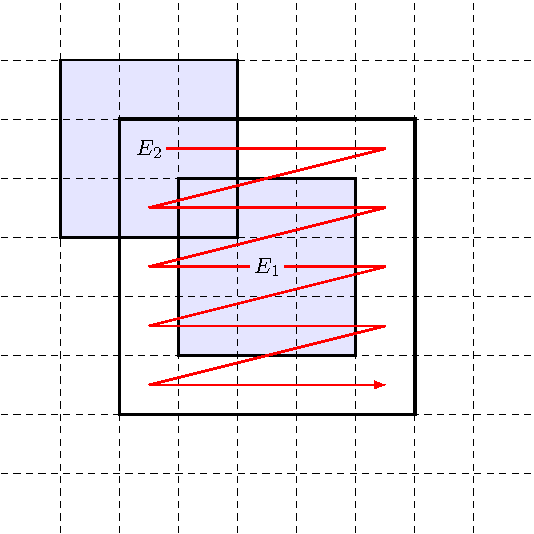
\includegraphics[scale=0.6]{../../Figures/Proyectos/UNGS2020/filtros.pdf}
%	\caption{Funcionamiento del algoritmo NLM}
%\end{figure}

Estos algoritmos proporcionan un marco general para el problema de reducción de este tipo de ruido dado que permiten proponer diferentes medidas de disimilaridad y diferentes pesos. 
Penna et al.~\cite{Penna2013} utilizaron la distancia de Kullback-Leibler en imágenes SAR monopolarimétricas para datos de intensidad, en reemplazo de la distancia euclídea que se utiliza en el algoritmo NLM original. 
Esta idea fue tomada por Santos et al.~\cite{Santos2017} y los autores la aplicaron en imágenes de ultrasonido que también están afectadas por ruido speckle. 
Xue et al.~\cite{Xue2013} reemplazan a la función de peso en el algoritmo NLM original por una combinación lineal de funciones cosenos obteniendo un algoritmo más rápido. 
Un nuevo filtro basado en distancias estocásticas y test entre funciones de distribución fue propuesto por Torres et al.~\cite{Torres2012} para datos SAR de intensidad.

El escenario planteado deja abierta la posibilidad de proponer distintas características de la imagen que sirvan de input para los algoritmos. Este proyecto propone estudiar la capacidad que tienen las medidas que provienen de la teoría de la información en la construcción de metodologías que puedan ser aplicadas tanto en la segmentación y clasificación de imágenes SAR, como en el diseño de nuevos métodos de filtrado.


%
%En este proyecto se estudiará la capacidad que tienen las medidas que provienen de la teoría de la información como atributos de una imagen SAR en el contexto del diseño de nuevos métodos de filtrado y de clasificación de imágenes SAR.

%\textcolor{red}{En algunos problemas de astroestadística se intenta hallar la función de densidad de una variable aleatoria $V$ desconocida a partir de una variable observada $Y$. Como ejemplo de esto se puede considerar a $V$ como la velocidad de rotación de las estrellas e $Y$ la proyección de la velocidad de rotación respecto  del eje de visión. Estas variables se relacionan a través de un modelo multiplicativo donde se plantea que $Y = V\cdot S$, siendo la distribución de $S$ perteneciente a una familia paramétrica conocida. Encontrar la función de densidad de $V$ se enmarca dentro de una importante clase importante de problemas denominados problemas de inversos, que tienen mucha aplicación en la astronomía como se presenta en el trabajo de Lucy~\cite{Lucy1994}. En Jorissen et al.~\cite{Jorissen2001} se presenta el modelo multiplicativo para la distribución de la masa en exoplanetas. En Curé et al.~\cite{Cure2014,Cure2015} los autores presentan un método para obtener la función de distribución acumulada de la velocidad de rotación de las estrellas y la del cociente de masas de estrellas binarias respectivamente, bajo el modelo multiplicativo. }
%
%\textcolor{red}{
%En la gran mayoría de los trabajos de la distribución de velocidades de rotación estelar se supone distribución uniforme de los ejes de rotación de las estrellas (similar suposición para sistemas binarios). Si bien esta hipótesis es ampliamente aceptada, algunos autores~\cite{Silva_2013, Rees2013} han puesto en duda este supuesto, como por ejemplo, cuando los ángulos de inclinación corresponden a estrellas en un cúmulo, debido a que los torques gravitacionales entre los miembros del cúmulo modifican la dirección de los ejes de rotación. Por lo tanto, es de interés estimar la función de densidad de la velocidad de rotación estelar bajo la suposición de una distribución de ejes de rotación no uniforme sobre la esfera.}
%
%\textcolor{red}{
%Tanto en el problema del modelo multiplicativo como en el análisis de espectrogramas, la variable de interés aparece en una ecuación de convolución. En esta propuesta se propondrán métodos basados en la minimización de distancias estocásticas como los utilizados en Cassetti et al.~\cite{Cassetti2020} con el objetivo de resolver el problema inverso para encontrar la función de densidad de la velocidad de rotación estelar.}



\section{Objetivos generales}

%La hip´otesis general de este proyecto es que es posible proponer modelos
%estad´ısticos que describan los datos de las im´agenes adecuadamente, de tal
%forma que, combinados con m´etodos de segmentaci´on, y con estimaciones muy
%precisas de los par´ametros lleven a la formulaci´on de metodolog´ıas y al desarrollo
%de t´ecnicas para la extracci´on de conocimiento a partir de datos muy complejos
%como son las im´agenes SAR Polarim´etricas. De esta forma es posible obtener
%contornos de regiones muy bien definidos, lo que mejorar´ıa en gran medida la
%interpretaci´on autom´atica de la misma.

%Este proyecto tiene como objetivo general profundizar en la utilización de medidas de \textcolor{red}{discriminación estocástica} que provienen de la teoría de la información que permitan tanto el desarrollo de nuevos métodos de clasificación basados en propiedades estadísticas del modelo considerado, como la implementación de nuevos métodos de filtrado  de imágenes para la reducción del ruido speckle.


\textcolor{red}{Este proyecto tiene como objetivo general profundizar en la utilización de medidas de discriminación estocástica que provienen de la teoría de la información en el procesamiento de imágenes y señales, con el fin de proponer modelos y técnicas estadísticas que describan los datos adecuadamente. Estas medidas junto con métodos de clasificación, de filtrado y de estimación de parámetros contribuirían a mejorar la interpretación de las imágenes y señales estudiadas.}


\section{Objetivos específicos}

Esta propuesta de investigación tiene por objetivos específicos:
\begin{itemize}
	\item Obtener expresiones explícitas de las $(h,\phi)$ entropías para el caso de la distibución $\mathcal{G}^0$.
	\item Implementar distintos estimadores de la entropía para el modelo $\mathcal{G}^0$ para datos de intensidad.
	\item Evaluar la performance de estos estimadores para muestras de tamaño pequeño y moderado incluyendo el análisis bajo contaminación.
	\item Generalizar este estudio para entropías $(h,\phi)$ como las definidas en~\cite{Menendez1997} y~\cite{Salicru1994}. 
	\item Evaluar la performance de algoritmos de clasificación tanto supervisada como no supervisada, considerando a la entropía como atributo de la imagen.
	\item Obtener herramientas robustas que puedan ser implementadas en el diseño de procedimientos resistentes bajo contaminación tales como algoritmos de clasificación y filtros de la clase Nonlocal Means.
	\item Extender estos procedimientos diseñados para imágenes SAR a otras disciplinas como la Astroestadística.
	\item Fortalecer el vínculo generado entre la Universidad de Valparaíso, Chile; University at Wellington, Nueva Zelanda y Universidad de Buenos Aires.
\end{itemize}

\section{Metodologías y fuentes}

Para alcanzar los objetivos planteados en este proyecto se propone iniciar esta investigación realizando un relevamiento de los distintos estimadores de la entropía de Shannon, un caso particular de las $(h,\phi)$ entropías, como los propuestos en~\cite{Beirlant1997,AlOmari2013,Behmardi2011} para el caso de la distribución $\mathcal{G}^0$ bajo el modelo multiplicativo.


%Este proyecto se basa en la hipótesis general que consiste en considerar a las $(h,\phi)$ entropías que, combinadas con la aplicación de filtros y métodos de clasificación permitan formular nuevas metodologías para la comprensión de imágenes SAR modelados con la distribución $\mathcal{G}^0$ bajo el modelo multiplicativo.


%Las imágenes SAR tienen muchas aplicaciones debido a sus ventajas respecto de las imágenes que provienen de sensores ópticos. La independencia de las condiciones climáticas y de la iluminación junto con la capacidad de penetrar la nubes, las copas de los árboles e incluso el suelo, han contribuido para que este tipo de imágenes resulten cada vez más populares.
%
%\textcolor{red}{\sout{Sin embargo, las imágenes SAR tienen la desventaja de ser difíciles de interpretar y procesar debido a la presencia del ruido speckle. Este ruido es inherente al proceso de captura de la imagen y se hace presente debido a la superposición coherente de las ondas reflejadas por muchos dispersores. Esto causa una variación en la intensidad píxel a píxel que se manifiesta en la imagen como un patrón granular. }}
%
%Debido a la aleatoriedad y a la fuerte dispersión que puede tener la señal retrodispersada, es necesario contar con modelos estadísticos que contribuyan a una mejor extracción de información a través del desarrollo de filtros, detección de bordes, clasificación de áreas entre otras metodologías. 

%El modelo multiplicativo es muy apropiado para explicar las características estadísticas de la imagen de un objeto cuando es iluminado por radiación coherente, como lo son las imágenes SAR.
%Este modelo considera que el valor observado en cada celda de la imagen es una variable aleatoria $Z$ que resulta del producto de dos variables aleatorias independientes: una correspondiente a la retrodispersión $X$ (que es lo que observaríamos sin la presencia del ruido speckle) y la otra correspondiente al ruido speckle $Y$ (que es inherente a todo sistema de captura de imágenes con iluminación coherente).

La clase de las $(h,\phi)$-entropías de una variable aleatoria $Z$ con función de densidad dada por $f_{Z}(z ; \boldsymbol{\theta})$ se definen como
\begin{align*}
H_{\phi}^{h}(\boldsymbol{\theta})=h\left(\int_{\mathcal{A}} \phi\left(f_{Z}(z ; \boldsymbol{\theta})\right) \mathrm{d} z\right),
\end{align*}
donde o bien se considera $\phi\colon [0, \infty) \rightarrow \mathbb{R}$ una función cóncava y $h\colon \mathbb{R} \rightarrow \mathbb{R}$ creciente, o $\phi$ convexa y $h$ decreciente. 
El cuadro~\ref{entropia} muestra algunas entropías presentadas en~\cite{Frery2019}.

\begin{table}[htb]
	\caption{\label{entropia} $(h,\phi)$ entropías}
	\centering
	\renewcommand*{\arraystretch}{2}
	\begin{tabular}{ccc} 
		\toprule
		$(h, \phi)$ -entropía & $h(y)$ & $\phi(x)$ \\
		\midrule 
		Shannon  & $y$ & $-x \ln x$ \\
		Rényi (orden $\left.\beta \in \mathbb{R}_{+}: \beta \neq 1\right)$ & $\dfrac{\ln y}{1-\beta}$ & $x^{\beta}$ \\
		Restricted Tsallis (orden $\left.\beta \in \mathbb{R}_{+}: \beta \neq 1\right)$ & $y$ & $\frac{x^{\beta}-x}{1-\beta}$ \\ 
		Arimoto de orden $\beta$ & $\dfrac{\beta-1}{y^{\beta}-1}$ & $x^{1 / \beta}$ \\ \addlinespace
		Sharma-Mittal de orden $\beta$ & $\dfrac{e^{(\beta-1) y}}{\beta-1}$ & $x \ln x$ \\
		\bottomrule
	\end{tabular}
\end{table}

%Bajo este modelo se pueden caracterizar regiones con diferente grado de textura a través de los parámetros de esta distribución. Para valores de $\alpha$ cercanos a cero (típicamente en el intervalo $(-3,0)$), la zona de la imagen corresponde a una región muy texturada, como es el caso de las zonas urbanas en las imágenes SAR. A medida que el valor del parámetro $\alpha$ disminuye, corresponde a zonas con cada vez menos textura, como son las regiones de forestación (usualmente $(-6,-3]$) y pastura (en $(-\infty,-6)$). Por otro lado, el parámetro $\gamma$ (llamado parámetro de escala) posee una interpretación en términos del brillo. Cuanto mayor es su valor, mayor intensidad posee la imagen en esa región. Por estas razones, la estimación precisa de los parámetros, en particular el parámetro de textura, es de suma importancia en el análisis de imágenes con ruido speckle. 

%En los últimos años se han propuesto varios métodos de estimación de parámetros, Vasconcellos et al.~\cite{VasconcellosFrerySilva:CompStat} cuantifican el error en la estimación del parámetro de textura para la distribución $\mathcal G_A^0$ y proponen una técnica analítica para mejorar la estimación.
%Silva et al.~\cite{SilvaCribariFrery:ImprovedLikelihood:Environmetrics} proponen otro método analítico para mejorar la estimación del parámetro de textura que reduce el error cuadrático medio.
%Cribari-Neto et al.~\cite{CribariFrerySilva:CSDA} proponen el uso de bootstrap para el mismo fin. 
%Allende et al.~\cite{AllendeFreryetal:JSCS:05} y Bustos et al.~\cite{BustosFreryLucini:Mestimators:2001} plantean mejoras para la estimación del parámetro de textura, pero con foco en su robustez. 

%Entre las técnicas de estimación paramétrica clásicas se encuentran las de máxima verosimilitud y momentos. Recientemente en~\cite{MellinAnalysisPolSAR,BujorTrouveValetNicolas2004,khan2014} han propuesto estimadores del parámetro de textura basado logcumulants y logmomentos, donde interviene la transforamda de Mellin de la función de densidad. En Tison et al.~\cite{Tison2004} los autores mostraron que los estimadors de los parámetros de la distribución $\mathcal G^0$, para datos de amplitud, mejoran al estimador de máxima verosimilitud.

%Como se dijo anteriormente es importante obtener estimadores que tengan un comportamiento adecuado para muestras de pequeño y moderado tamaño tanto en sesgo, error cuadrático medio como en robustez. Tanto de los parámetros de la distribución como de los atributos de las imágenes. Esto es importante en el procesamiento de imágenes ya que muchos de los métodos de filtrado de imágenes, detección de bordes y clasificación utilizan máscaras deslizantes de tamaño $3 \times 3$,  $5 \times 5$, $7 \times 7$, $9 \times 9$ o $11 \times 11$. 

En  relación con el modelo multiplicativo se plantea que el retorno se modela como el producto de dos variables aleatorias independientes $X$ e $Y$, la primera corresponde al backscatter o retrodispersión y la segunda al ruido speckle. 
De esta forma $Z=X\cdot Y$ representa el retorno en cada pixel bajo el modelo multiplicativo.
El ruido speckle $Y$, en formato intesidad, se modela por la distribución gama de media unitaria y parámetros $(L,L)$, donde con $L\geq 1$ es el número de looks que indica la relación señal/ruido de la imagen. 
El backscatter $X$ se describe por una distribución gama Inversa de parámetros $(-\alpha ,\gamma)$. 
De esta forma tenemos que $Z$ obedece a una distribución $\mathcal G^0$ con función de densidad 	dada por
\begin{equation*}
f_{\mathcal{G}^{0}}( z) =\frac{L^{L}\Gamma ( L-\alpha
	) }{\gamma ^{\alpha }\Gamma ( -\alpha ) \Gamma (
	L) }\cdot  
\frac{z^{L-1}}{( \gamma +zL) ^{L-\alpha }},%
\label{ec_dens_gI0}
\end{equation*}
donde $-\alpha,\gamma ,z>0$ y $L\geq 1$.

Los momentos de orden $r$ están expresados por
\begin{equation*}
E\left(Z^{r}\right)=\left(\frac{\gamma}{L}\right)^{r} \frac{\Gamma(-\alpha-r)}{\Gamma(-\alpha)} \frac{\Gamma(L+r)}{\Gamma(L)}
\end{equation*}
y son finitos si $\alpha<-r$. Condición que se tiene en cuenta al momento de hacer el estudio.


 Teniendo en cuenta la expresión explícita de la entropía de Shannon dada en Ferrerira et al.~\cite{Ferreira2020} para el caso de la función de densidad $\mathcal{G}^0$ y, combinando con los resultados obtenidos en Cassetti et al.~\cite{Cassetti2020} en cuanto a la estimación del parámetro de textura, se implementarán estos estimadores y se estudiará la performance de los mismos a través de simulaciones Montecarlo donde se:
\begin{itemize}
	\item Considerará un espacio paramétrico que contemple distintas texturas, distintos números de looks y tamaño de muestra.
	\item Estudiará el sesgo, error cuadrático medio de los mismos.
	\item Analizará su robustez, es decir, su comportamiento bajo corrimientos del modelo teórico. 
	\item Evaluará su costo computacional.
\end{itemize} 

%Se extenderá este estudio a otras entropías definidas dentro de la familia $(h,\phi)$ como las que se presentan en dadas en el cuadro~\ref{entropia}.

Un segundo paso es el diseño e implementación de nuevos procedimientos robustos para reducir la presencia del ruido speckle como, por ejemplo, los filtros NLM. En esta clase de filtros el valor del píxel estimado se obtiene como un promedio ponderado donde el peso de cada píxel en la imagen original es proporcional a una medida de similaridad entre los píxeles que se encuentran en
un entorno ($E_1$) del píxel de referencia y los píxeles pertenecientes a un entorno ($E_2$) de los alrededores de $E_1$. La figura~\ref{NLM} tomada de Penna et al.~\cite{Penna2013} muestra un esquema del funcionamiento de este algoritmo. 

\begin{figure}[hbt]
	\label{NLM}
	\centering
	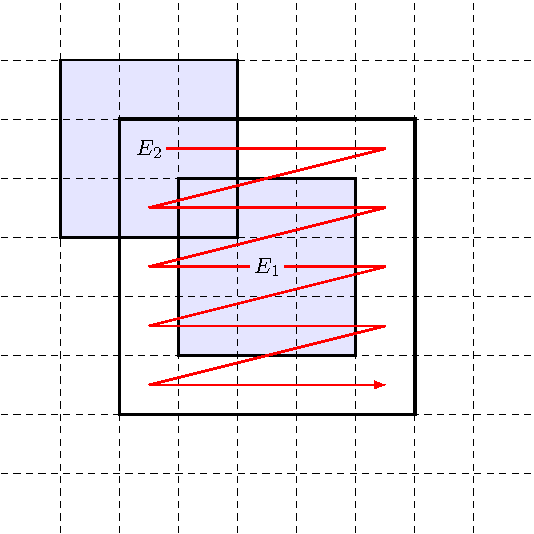
\includegraphics[scale=0.6]{../../Figures/Proyectos/UNGS2020/filtros.pdf}
	\caption{Funcionamiento del algoritmo NLM}
\end{figure}

Se utilizarán los resultados obtenidos del estudio y análisis de los diferentes estimadores de la entropía para proponer una medida de similaridad entre píxeles. Se comparará el desempeño de esta propuesta con las que existen en la literatura a través de diferentes medidas como las que se indican en~\cite{Frery2019}.

Asimismo, serán estudiados algoritmos de clasificación tanto supervisados como no supervisados, para generar mapas temáticos de imágenes SAR utilizando medidas de disimilaridad en combinación con métodos de filtrado. 
Estos algoritmos serán comparados con los existentes en la literatura a través de diferentes indicadores como los son el índice Kappa y la matriz de confusión.

La efectividad de todos estos procedimientos será evaluada aplicándolos a imágenes reales.

%\textcolor{red}{
%En cuanto a la aplicación de estas medidas a problemas de deconvolución en astroestadística, el problema que se quiere abordar puede ser formulado de la siguiente forma:
%Sea $V$ una variable aleatoria continua con función de densidad dada por $f_{V}$ desconocida. Sea $Y=V . S$ donde $S$ es una variable aleatoria con distribución conocida. Se quiere conocer la distribución de la variable aleatoria $V$ a partir de una muestra de la variable aleatoria $Y$. A partir del teorema del cambio de variables y de la suposición de independencia entre $\mathrm{V}$ y $\mathrm{S}$, se obtiene una expresión que relaciona las densidades de las variables involucradas:
%}
%\begin{align}
%\label{Fredholm}
%f_{Y}(y)=\int_{y}^{\infty} \dfrac{1}{v} f_{S}(y \vert v) f_{V}(v) d v
%\end{align}
%
%Si llamamos $p(y \vert v)=\dfrac{1}{v} f_{S}(y \vert v)$ se obtiene una ecuación integral de Fredholm de primera especie siendo $p(y \vert v)$ el kernel de la integral.
%Si se supone que $V$ es la velocidad de rotación estelar y $S=\sin i$ donde $i$ es el ángulo de inclinación respecto a la línea de visión, por~\eqref{Fredholm} se obtiene una ecuación que relaciona la distribución de las velocidades proyectadas con la distribución de las velocidades verdaderas.
%
%En los últimos tiempos la suposición de que los ejes no se distribuyen uniformemente sobre la esfera está en discusión como es el caso de los cúmulos estelares.
%En estas situaciones es razonable considerar la suposición de correlación entre los ejes de rotación, es decir suponer que los ejes de rotación se distribuyen con una dirección preferencial.
%
%En este sentido la propuesta de este proyecto es generalizar la integral de Fredholm de la ecuación~\eqref{Fredholm}, asumiendo que los ejes de rotación estelar distribuyen con una función $\mathrm{H}$. De esta forma~\eqref{Fredholm} queda expresado como
%\begin{align}
%f_{Y}(y)=\int_{y}^{\infty}\dfrac{1}{x} H\left(\sqrt{1-y^{2} / x^{2}}\right) \frac{y}{\sqrt{x^{2}-y^{2}}} f_{X}(x) d y.
%\end{align}
%La función de distribución $\mathrm{H}$ modela la distribución de los ejes de rotación, que tiene como caso particular a~\eqref{Fredholm} cuando $\mathrm{H}=1$, correspondiendo a la distribución uniforme de ejes. 
%
%En esta generalización se aboradará el problema desde un punto de vista paramétrico considerando conocido el modelo para las velocidades de rotación estelar y se analizarán varias situaciones:
%\begin{itemize}
%	\item En una primera aproximación se asumirá que las velocidades de rotación estelar están descritas por una distribución Maxwelliana de parámetro $\lambda$, modelo ampliamente utilizado en la literatura.
%	\item En una segunda instancia se considerará a las distribuciones de Kaniadakis$(k)$ y Tsallis$(q)$~\cite{Carvalho2009}, ya que éstas ajustan bien a la distribución de velocidades bajo el supuesto de uniformidad.
%\end{itemize} 
%
%Por otro lado se propone modelar a la distribución de los ejes de rotación como una distribución $Beta(\alpha,\beta)$ porque incluye tanto el caso uniforme como el de pequeñas perturbaciones respecto de una dirección privilegiada y tiene como caso particular al caso uniforme. 
%
%Con estas consideraciones los parámetros estimados del modelo se obtendrían a través de la minimización de una distancia estocástica entre lo derivado de la convolución y un estimador por núcleos de la función de densidad de las velocidades proyectadas observadas.
\textcolor{red}{
En muchos problemas de astrofísica se intenta hallar la distribución de una variable aleatoria $X$ a partir de una variable observada $Y$ relacionada de la forma $Y = S\,X$, donde la distribución de $S$ pertenece
a una familia paramétrica conocida. Esta clase de problemas, conocida como problemas inversos, son ampliamente utilizados en astroestadística como se indica en el trabajo de Lucy~\cite{Lucy1994}. La distribución de la masa en exoplanetas~\cite{Jorissen2001},  de la velocidad de rotación de las estrellas y del cociente de masas de estrellas binarias~\cite{Cure2014,Cure2015} son ejemplos de aplicación de este modelo.
}

\textcolor{red}{
En lineas generales, los métodos utilizados para abordar este problema se basan en la minimización de la distancia entre una estimación de la función de densidad $f_{Y}$ observada y la $f_{Y}$ derivada del modelo. 
En este proyecto se propone analizar la eficiencia de estas distancias estocásticas a través de simulaciones MonteCarlo. En una segunda instancia se aplicarán estos métodos a problemas con datos reales.
}
%se propone minimizar la distancia de la $Y$ observada y la obtenida por el algoritmo.
%Se propone analizar la eficiencia de distancias estocásticas en comparación a los métodos usuales y proponer métodos óptimos
%\begin{itemize}
%	\item Simular distribuciones de $X$ aplicar los algoritmos de minimización y comparar los resultados.
%	\item Aplicar dichos métodos a problemas reales y comparar con los métodos estándar.
%\end{itemize}
% 


%Cabe señalar que la ecuación~\eqref{Fredholm} se puede llevar (vía discretización) a una forma matricial del tipo:
%\begin{align}
%Z=A . T
%\end{align}
%
%en donde $Z$ representa a la función de densidad de los datos observados $f_{Y},$ mientras que $A$ representa al término $p(y \vert v)$ y T representa a la función de densidad de las velocidades de rotación estelar $f_{V}$. Matemáticamente la ecuación (1) representa un problema mal planteado (ill-possed problem), en donde pequeños errores de medición pueden producir grandes variaciones en los datos recuperados entregando resultados inestables .
%
%En lineas generales, los métodos buscan la distribución $F_{X}$ tal que la distancia de $F_{y}$ a la distribución observada
%sea mínima. Las distancias consideradas en general son variaciones de mínimos cuadrados.
%En los métodos propuestos se busca minimizar la distancia de la $Y$ observada y la obtenida por el algoritmo.
%Se propone analizar la eficiencia de distancias estocásticas en comparación a los métodos usuales y proponer métodos óptimos
%\begin{itemize}
%	\item Simular distribuciones de $X$ aplicar los algoritmos de minimización y comparar los resultados.
%	\item Aplicar dichos métodos a problemas reales y comparar con los métodos estándar.
%\end{itemize}


\section{Actividades y cronograma}

\subsection{Actividades}

Para alcanzar los objetivos planteados se proponen las siguientes actividades:
\begin{enumerate}
	\item Realizar un relevamiento de trabajos de investigación de estimadores de la entropía de Shannon, en particular aplicados a imágenes SAR.
	\item Implementar diferentes estimadores de la entropía de Shannon de la distribución $\mathcal{G}^{0}$ de acuerdo al relevamiento realizado en el item anterior. Producción de rutinas.
	\item Evaluar, a través de simulaciones MonteCarlo y estudiando el sesgo y error cuadrático medio, el desempeño de estos estimadores para diferentes combinaciones de los parámetros de la distribución $\mathcal{G}^{0}$, consideraránerando distintos tamaños de muestra y su robustez.
	%\item Evaluar la resistencia a la contaminación por corner reflector de los estimadores 	propuestos utilizando técnicas de MonteCarlo.
	\item \textcolor{red}{Estudiar el desempeño que tienen diferentes distancias estocásticas en la estimación de parámetros de la distribución de la velocidad de rotación de estrellas bajo el modelo multiplicativo.}
	\item Encontrar expresiones explícitas de diferentes entropías de la distribución $\mathcal{G}^{0}$.
	\item Extender el estudio realizado en los ítems 1) a 4) para diferentes entropías.
	\item Realizar un relevamiento de trabajos de investigación que traten del diseño, implementación y aplicaciones de filtros del tipo NLM en imágenes SAR.
	\item Proponer e implementar nuevos métodos de filtrado de imágene SAR del tipo NLM considerando a las diferentes entropías  como medida de distancia. Producción de rutinas.
	%\item Implementar estos filtros NLM considerando a las diferentes entropías  como medida de distancia. Producción de rutinas.
	\item Evaluar el desempeño de estos filtros tanto en imágenes simuladas como en reales  y compararlos con otros filtros existentes en la literatura.
	\item Realizar un relevamiento de trabajos de investigación que contemple el diseño e implementación de algoritmos de clasificación utilizando distintos atributos de las imágenes SAR.
	\item Proponer e implementar nuevos métodos de clasificación, con y sin la utilización de filtros, en imágenes sintéticas y reales. Evaluación de la performance de estos métodos y producción de rutinas.
	\item Documentación y publicación de resultados.
	
\end{enumerate}

\subsection{Cronograma}
El cronograma de trabajo se muestra en los siguientes cuadros:

\begin{table}[htb]
	\caption{\label{entropia} Cronograma de actividades del Año 2021}
	\centering
	\renewcommand*{\arraystretch}{2}
\begin{tabular}{ccccccccccccc}
	\toprule
	\multirow{2}{*} {Actividades} & \multicolumn{12}{c} { Meses  } \\
	\cmidrule(){2-13}
	& 1 & 2 & 3 & 4 & 5 & 6 & 7 & 8 & 9 & 10 & 11 & 12 \\
	\midrule
	  1-4 & $\mathrm{x}$ & $\mathrm{x}$ & $\mathrm{x}$ & $\mathrm{x}$ & $\mathrm{x}$ & & & & & & & \\
	\hline 
	5, 6  & & & & $\mathrm{x}$& $\mathrm{x}$ & $\mathrm{x}$  & $\mathrm{x}$ & $\mathrm{x}$ &  & & & \\
	\hline 12 & & & & & & & & $\mathrm{x}$ & $\mathrm{x}$ & $\mathrm{x}$ & $\mathrm{x}$ & $\mathrm{x}$ \\
	\hline
\end{tabular}
\end{table}


\begin{table}[htb]
	\caption{\label{entropia} Cronograma de actividades del Año 2022}
	\centering
	\renewcommand*{\arraystretch}{2}
	\begin{tabular}{ccccccccccccc}
		\toprule
		\multirow{2}{*} {Actividades} & \multicolumn{12}{c} { Meses  } \\
		\cmidrule(){2-13}
		& 1 & 2 & 3 & 4 & 5 & 6 & 7 & 8 & 9 & 10 & 11 & 12 \\
		\midrule
		7, 8 y 9 & $\mathrm{x}$ & $\mathrm{x}$ & $\mathrm{x}$ &  &  & & & & & & & \\
		\hline 
		10 y 11  & & & & $\mathrm{x}$& $\mathrm{x}$ & $\mathrm{x}$  & $\mathrm{x}$ &  &  & & & \\
		\hline 12 & & & & & & & & $\mathrm{x}$ & $\mathrm{x}$ & $\mathrm{x}$ & $\mathrm{x}$ & $\mathrm{x}$ \\
		\hline
	\end{tabular}
\end{table}

\section{Contribuciones}

Como resultado de esta investigación se espera:

\begin{enumerate}
	\item Proponer métodos de estimación de entropías para la distribución $\mathcal{G}^0$ que sean robustos ante desvíos del modelo teórico.
	\item Implementar rutinas de estimación de entropías para la distribución $\mathcal{G}^0$.
	\item Proponer algoritmos que permitan estimar la distribución de velocidades de rotación de las estrellas.
	\item Proponer métodos de filtrado de la clase NLM utilizando medidas de entropía en imágenes SAR con datos de intensidad.
	\item Implementar y generar rutinas para la aplicación de los métodos de filtrado propuestos.
	\item Desarrollar métodos de clasificación de imágenes SAR utilizando medidas de entropía como atributo para clasificar.
	\item Implementar y generar rutinas para la aplicación de métodos de clasificación en imágenes SAR. Estos métodos pueden estar combinados con los métodos NLM para la reducción del ruido speckle.
	\item Proponer métodos de estimación de la velocidad de rotación de ciertos grupos de estrellas.
	\item Producción de artículos científicos que serán enviados a revistas internacionales de alto impacto. 
\end{enumerate}

\section{Relación con la docencia}

Este proyecto se articula con la materia Estadística del
Profesorado Universitario de Educación Superior en Matemática. Temas centrales como los son métodos de estimación y propiedades de los estimadores forman parte del programa. Asimismo el uso del software R project, con el que se trabajará en este proyecto, es de uso permanente en esta materia.
La directora del proyecto junto con Gustavo Paccosi participan regularmente del dictado de Estadística. Daiana Delgadino tuvo beca de docencia y de docencia e investigación en la materia Estadística bajo la dirección de la directora del proyecto y actualmente participa regularmente en el dictado de la materia Lógica y Teoría de Números. Melina Sarni tuvo beca de docencia en la materia Estádistica también bajo la dirección de la directora del proyecto. Actualmente participa regularmente del dictado de los Talleres Iniciales Orientados en Ciencias Exactas. También participó del dictado de la materia Estadística durante el segundo semestre del 2019.   

Cabe señalar que las ediciones de la Escuela de Matemática de Invierno - Sabrina Victoria Vieiro (EMASUNGS) de los años $2017$, $2018$ y $2019$ contó  con el dictado de un curso de simulación utilizando el software R project de uso en la materia Estadística. Este curso fue diseñado y dictado por la directora del proyecto en colaboración con los integrantes Gustavo Paccosi, Daiana Delgadino y Melina Sarni en los dos primeros años. 

Durante el año $2019$ Alejandro Frery, integrante del proyecto, visitó la universidad en el marco de la \textit{Movilidad de Investigadores Invitados en la UNGS – MOVIUNGS 2018/2019} y dictó un curso para alumnos del Doctorado en Ciencia y Tecnología de la Universidad en procesamiento de imágenes SAR, y dió una charla orientada a los alumnos de grado del  Profesorado Universitario de Educación Superior en Matemática en algunos tópicos de Estadística.  


%La implementación de los algoritmos propuestos serán desarrollados en 
%comparaci´on de los m´etodos de segmentaci´on basados en contornos combinados
%con la estimaci´on de los par´ametros
%
%Formulación de algoritmos para calcular nuevos estimadores de
%los par´ametros que sean robustos, implementaci´on computacional de los mismos
%y aplicaci´on a im´agenes sint´eticas y reales. Luego, medir el error que se comete
%al aplicarlos y comparar con diferentes m´etodos ya existentes en la literatura.
\bibliographystyle{unsrt}
\bibliography{../../Bibliography/bib_julia2,../../Bibliography/bib_julia_Astro}



\end{document}
